\documentclass[a4paper]{article} % set paper size

\usepackage[utf8]{inputenc}
\usepackage {url}
\usepackage[top=2.0cm, bottom=2.0cm, left=2.54cm, right=2.54cm]{geometry} % set margin
\usepackage{amsfonts} % for set names
\usepackage{amsmath} % for equation system
\usepackage{amsthm} % for theorem block
\usepackage{fixltx2e} % for subscript
\usepackage{fancyhdr} % for footer/headline modification
\usepackage{xcolor}
\usepackage{graphicx,float} % for image insertion
\usepackage{multicol} %for text in tow columns

\usepackage{wrapfig} %figure wrapping


\pagestyle{fancyplain} % for footing modification on all pages
\fancyhf{}
%\renewcommand{\headrulewidth}{0pt} % remove decorative lign

\fancyhead[L]{Pauline Maury Laribiere\\
              Alexandre Devienne}
\fancyhead[R]{MT/EL-BA2 EPFL \\
                \today}
\fancyhead[C]{\textbf{Spring programming project : Microcosmos}}

\fancyfoot[R]{\thepage\ of \pageref{lastpage}}

\begin{document}
\begin{multicols*}{2}
% =====================================================================
\section{Program's architecture}


\begin{figure}[H]
\centering
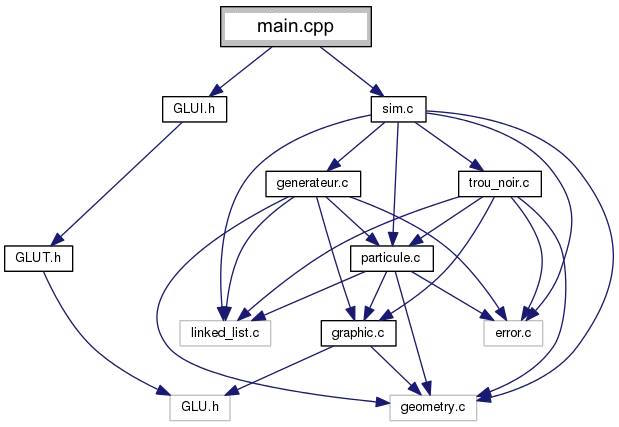
\includegraphics[width=0.48\textwidth]{architecture.jpg}
\caption{Final architecture}
\end{figure}


Compared to the architecture suggested, we added two low level modules, and 2 dependencies:
\begin{description}
\item[Module: geometry.]
Low level representation of points and vectors and functions to manipulate them (ex: distance between points, norm of a vector)

%This module in included in the modules : \emph{main}, \emph{sim}, \emph{generateur}, \emph{particule}, \emph{trou\_noir}, \emph{graphic}.

\item[Module: linked\_list.]
Generic double linked list data structure.
Some basic dictionary operations are implemented such as : first, next, add, delete, search.
More complex operations exist such as : sorting and calling a function with 2 elements as arguments, for every possible 2-combinations of elements
(to work out the forces between every particles for example)

%This module in included in the modules : \emph{sim}, \emph{generateur}, \emph{particule}, \emph{trou\_noir}.

\item[Dependency: trou\_noir $\rightarrow$ particule.]
This allows \emph{trou\_noir} to call \texttt{part\_applyForceField( void (*forceFieldAt) (POINT p) )}
to apply the force generated by all black holes to all particles.
Plus, to destroy particles too close to a black hole, it can call \texttt{int part\_closestPartOn( POINT p )}
to retrieve a particle's ID to then destroy it with: \texttt{part\_delete( int partID )}

\item[Dependency: generateur $\rightarrow$ particule.]
This allows \emph{generateur} to delegate the validity of a generator's arguments to \emph{particule}
(using \texttt{part\_validParams}) 
and to create new particles by a simple call of \texttt{part\_create}
(but first call \texttt{part\_closestPartOn} to check if a particle covers the generator)
\end{description}

Working with these modules eases our work by reducing the amount of redundant code and delegating complex generic tasks
(such as adding an element to a linked list or working out a linear interpolation) to specialized modules.
It also eased the testing part, as we could validate the correctness of these modules before using them in the project.

% =====================================================================
\section{Data structures}

To store the data from the particles, generators and black holes,
we used arrays of size MAX\_RENDU1 for the \emph{rendu 1}.
But for the \emph{rendu 2} we needed a way to store large numbers of entities,
without any knowledge of the maximum amount.
We first consider arrays which double in size when full, but it has 2 drawbacks :
spikes in calculation time (when the array is re-allocated)
and a possibility that half the allocated memory isn't used (possibly even more if some elements are deleted)

To avoid these drawbacks we had little choice but to use \emph{linked lists}.
Because we were going to use linked lists for the particles, generators and black holes, to avoid redundant code,
we decided to write a generic double linked list module.

This module handles all the hassle of creating and deleting dynamically elements.

%This even allowed us to code some complex behaviour in the module that we could later use with a simple function call
%(ex: search, sort or even applying a function to all elements), without any \texttt{while} or \texttt{for} loop to write.


% =====================================================================
\section{Function called by \emph{main.cpp} from \emph{sim.c}}
Here are the different functions of \emph{sim.c} called in \emph{main.cpp} :

\begin{itemize}
\item Beginning and saving a simulation:
    \begin{itemize}
    \item \texttt{sim\_openFile}: begin a new simulation from a given file and mode
    \item \texttt{sim\_save}: save the current state of the simulation in a file
    \end{itemize}
\item Getting information from the simulation:
    \begin{itemize}
    \item \texttt{sim\_nbEntities}: get the number of each entity (to display in GLUI)
    \item \texttt{sim\_extremPoints}: return the outermost points of the simulation to calculate the frame of the window to open
    \end{itemize}
\item Handling the advancement of the simulation:
    \begin{itemize}
    \item \texttt{sim\_display}: display the current state of the simulation (with all the entities) 
    \item \texttt{sim\_next\_step}: calculate the simulation's next step
    \end{itemize}
\item Handling the user inputs:
    \begin{itemize}
    \item \texttt{sim\_select}: enables the user to select an entity
    \item \texttt{sim\_deleteSelection}: delete the selected entity
    \item \texttt{sim\_deselect}: deselect the current selection
    \end{itemize}
\item Exiting a simulation:
    \begin{itemize}
    \item \texttt{sim\_clean}: free all the memory allocated to all the simulation sub-modules
    \end{itemize}
\end{itemize}



\label{lastpage}
\end{multicols*}
\end{document}
